\documentclass[aspectratio=169]{beamer}
\usepackage[utf8]{inputenc}
\usepackage[T1]{fontenc}
\usepackage{svg}
\usepackage{todonotes}
\usepackage{siunitx}
\usepackage{tikz}
\usepackage{pgfplots}
\usepackage{eurosym}
\usepackage{relsize}
\usepackage{ellipsis}
\usepackage{listings}
\usepackage{subcaption}

\pgfplotsset{compat=newest} % Allows to place the legend below plot
\usepgfplotslibrary{units} % Allows to enter the units nicely

\setbeamertemplate{caption}[numbered]

% https://tex.stackexchange.com/questions/99316/symbol-for-external-links/294990#294990
\newcommand{\ExternalLink}{%
    \tikz[x=1.2ex, y=1.2ex, baseline=-0.05ex]{% 
        \begin{scope}[x=1ex, y=1ex]
            \clip (-0.1,-0.1) 
                --++ (-0, 1.2) 
                --++ (0.6, 0) 
                --++ (0, -0.6) 
                --++ (0.6, 0) 
                --++ (0, -1);
            \path[draw, 
                line width = 0.5, 
                rounded corners=0.5] 
                (0,0) rectangle (1,1);
        \end{scope}
        \path[draw, line width = 0.5] (0.5, 0.5) 
            -- (1, 1);
        \path[draw, line width = 0.5] (0.6, 1) 
            -- (1, 1) -- (1, 0.6);
        }
    }

\newcommand\Colorhref[3][structure.fg]{\href{#2}{\color{#1}#3 \ExternalLink}}

\title{Open Data: \\ Receive it Yourself}
\date[ISPN ’80]{Datenspuren 2022, Dresden}
\author[]{Tassilo, 0xA, Marenz (dump@dvb.solutions)}

\usetheme{dvb}

\AtBeginSection[]{
  \begingroup
  \setbeamertemplate{background}{
    \begin{tikzpicture}
      \useasboundingbox (0,0) rectangle(\the\paperwidth,\the\paperheight);
      \fill[dvbyellow,rotate around={70:(0,0)}] (0,-2) rectangle (22,0);
      \fill[dvbyellow,rotate around={70:(3,0)}] (0,-2) rectangle (22,0);
    \end{tikzpicture}
  }
  \begin{frame}
  \vskip4cm%
    \begin{beamercolorbox}[wd=12cm,leftskip=3cm]{title page header}
    	\usebeamerfont{title}\textbf{\LARGE \fontfamily{pag}\selectfont \secname}\par%
    \end{beamercolorbox}
  \vfill
  \end{frame}
  \endgroup
}

\newcommand*{\myfont}{\fontfamily{pag}\selectfont}

\makeatletter
\tikzset{
    database/.style={
        path picture={
            \draw (0, 1.5*\database@segmentheight) circle [x radius=\database@radius,y radius=\database@aspectratio*\database@radius];
            \draw (-\database@radius, 0.5*\database@segmentheight) arc [start angle=180,end angle=360,x radius=\database@radius, y radius=\database@aspectratio*\database@radius];
            \draw (-\database@radius,-0.5*\database@segmentheight) arc [start angle=180,end angle=360,x radius=\database@radius, y radius=\database@aspectratio*\database@radius];
            \draw (-\database@radius,1.5*\database@segmentheight) -- ++(0,-3*\database@segmentheight) arc [start angle=180,end angle=360,x radius=\database@radius, y radius=\database@aspectratio*\database@radius] -- ++(0,3*\database@segmentheight);
        },
        minimum width=2*\database@radius + \pgflinewidth,
        minimum height=3*\database@segmentheight + 2*\database@aspectratio*\database@radius + \pgflinewidth,
    },
    database segment height/.store in=\database@segmentheight,
    database radius/.store in=\database@radius,
    database aspect ratio/.store in=\database@aspectratio,
    database segment height=0.1cm,
    database radius=0.25cm,
    database aspect ratio=0.35,
}
\makeatother

\begin{document}

\begin{frame}\titlepage
\end{frame}
  
\begin{frame} 
 %\includesvg{dvbdump}
\frametitle{Roadmap} 
%\framesubtitle{The proof uses \textit{reductio ad absurdum}.} 

\tableofcontents

\end{frame}

% =================================================

\section{Radio \& VDV 420}

% =================================================

% =================================================

\begin{frame}
\frametitle{Data Sources}
\framesubtitle{Overview of Traffic Light Control (Ampelbeeinflussung)}
\begin{figure}
\centering
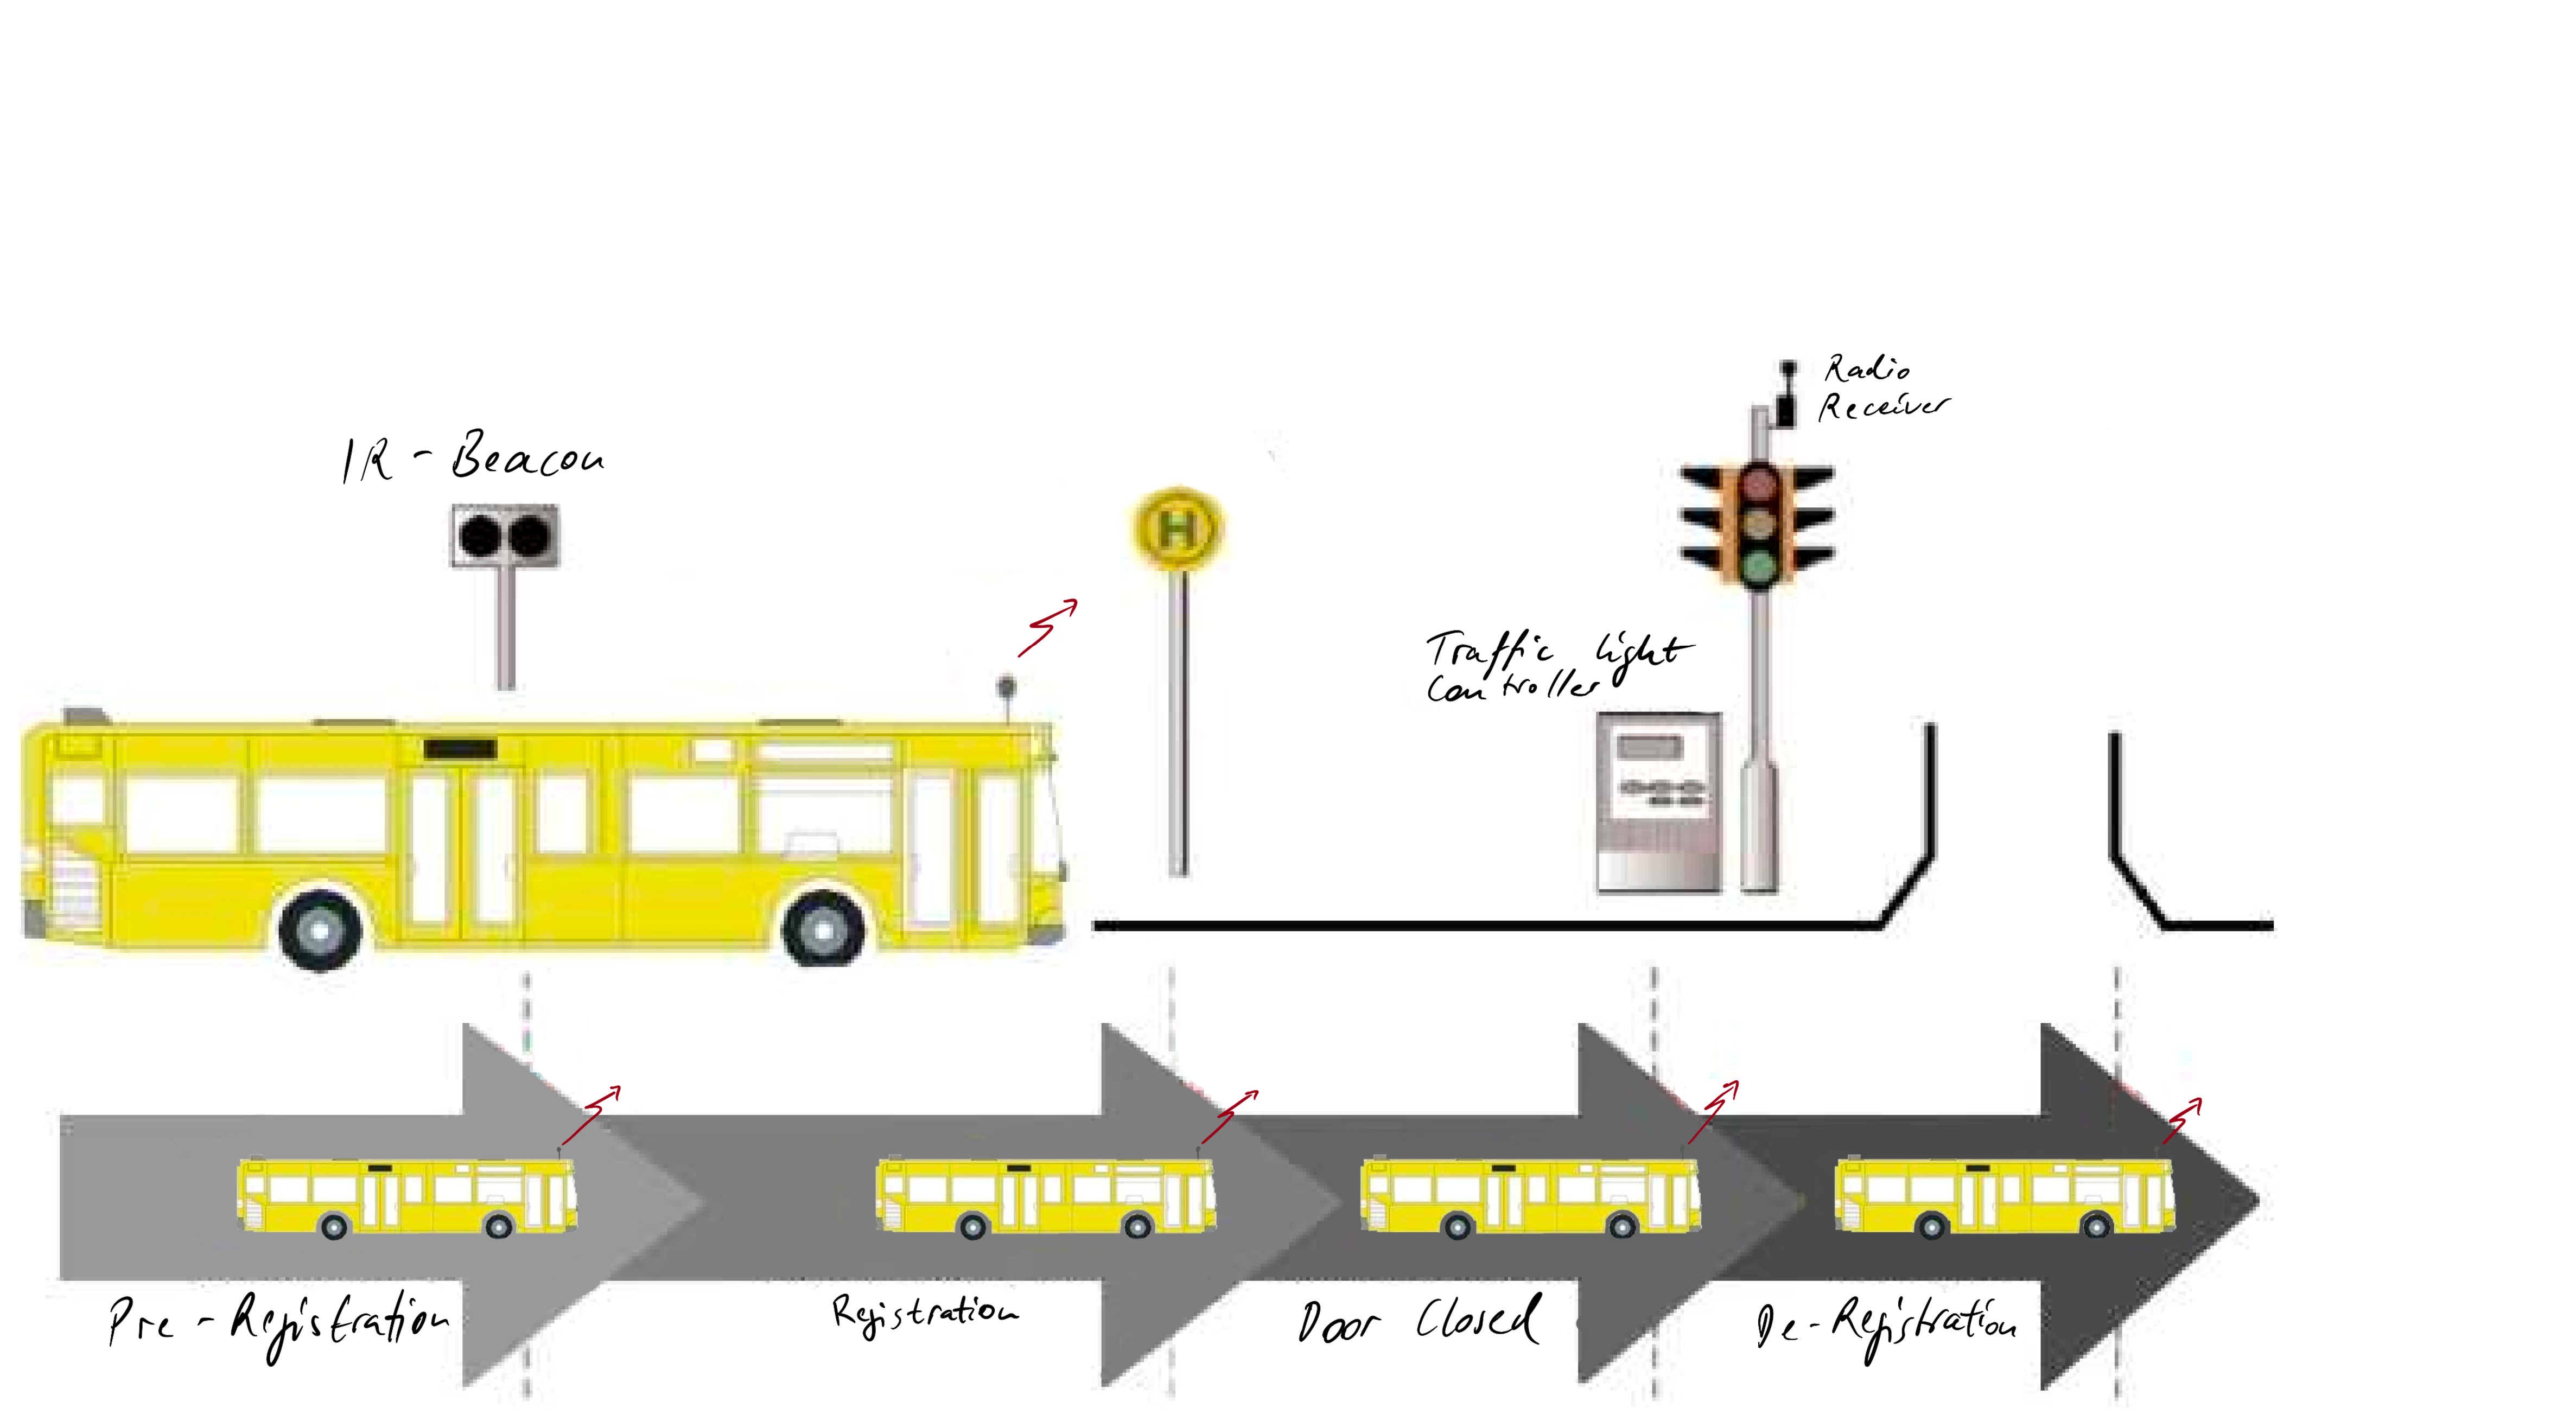
\includegraphics[height=0.65\textheight]{figs/lsa-beeinflussungs-stecke.pdf}
\caption{Traffic light controlled by radio link of busses and trams. Modified graphic from \Colorhref{https://urbic-system.com/wp-content/uploads/2020/10/Qualitaetssicherung-an-Lichtsignalanlagen-aus-Sicht-des-OEPNV-im-urbanen-Umfeld-Kopie.pdf}{urbic}}
\end{figure}
\end{frame}

% =================================================

\begin{frame}
\frametitle{Data Sources}
\framesubtitle{Overview of Traffic Light Control (Ampelbeeinflussung)}
\begin{figure}
\centering
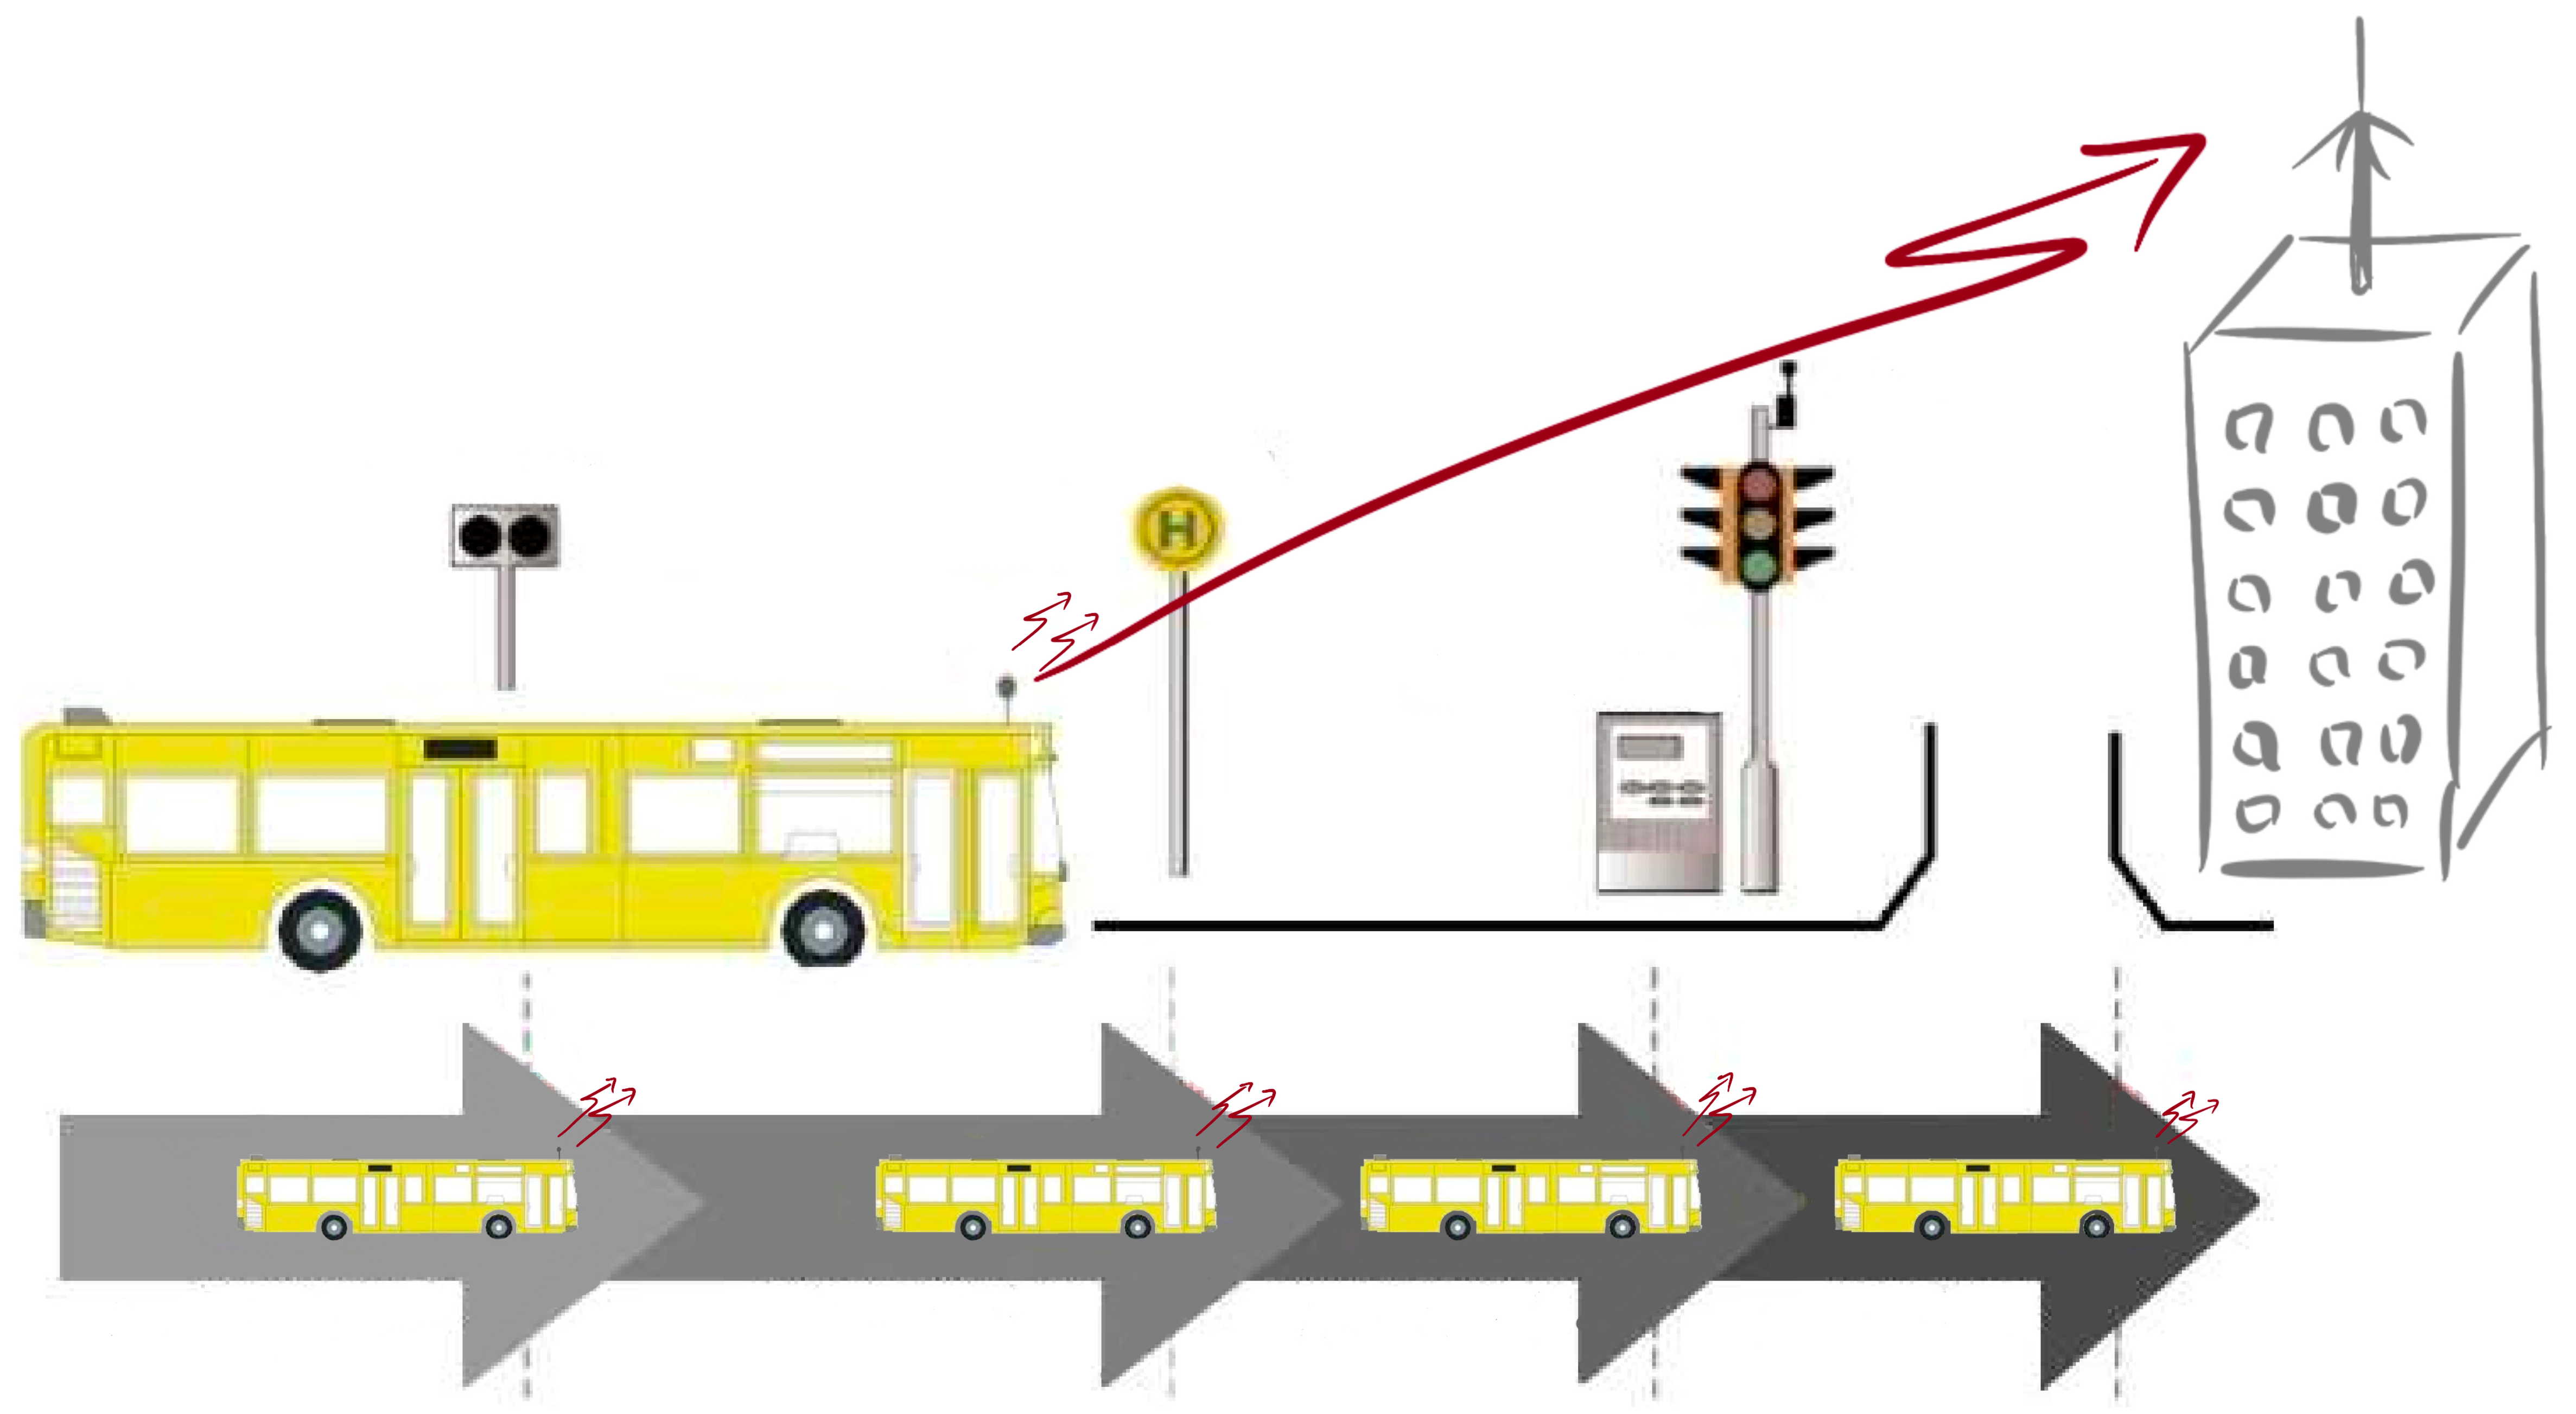
\includegraphics[height=0.65\textheight]{figs/lsa-beeinflussungs-stecke-mit-antenne.pdf}
\caption{Radio signals can be received by our antennas}
\end{figure}
\end{frame}

% =================================================

\begin{frame}
\frametitle{Data Sources}
\framesubtitle{Receiver Overview}
\begin{figure}
\centering
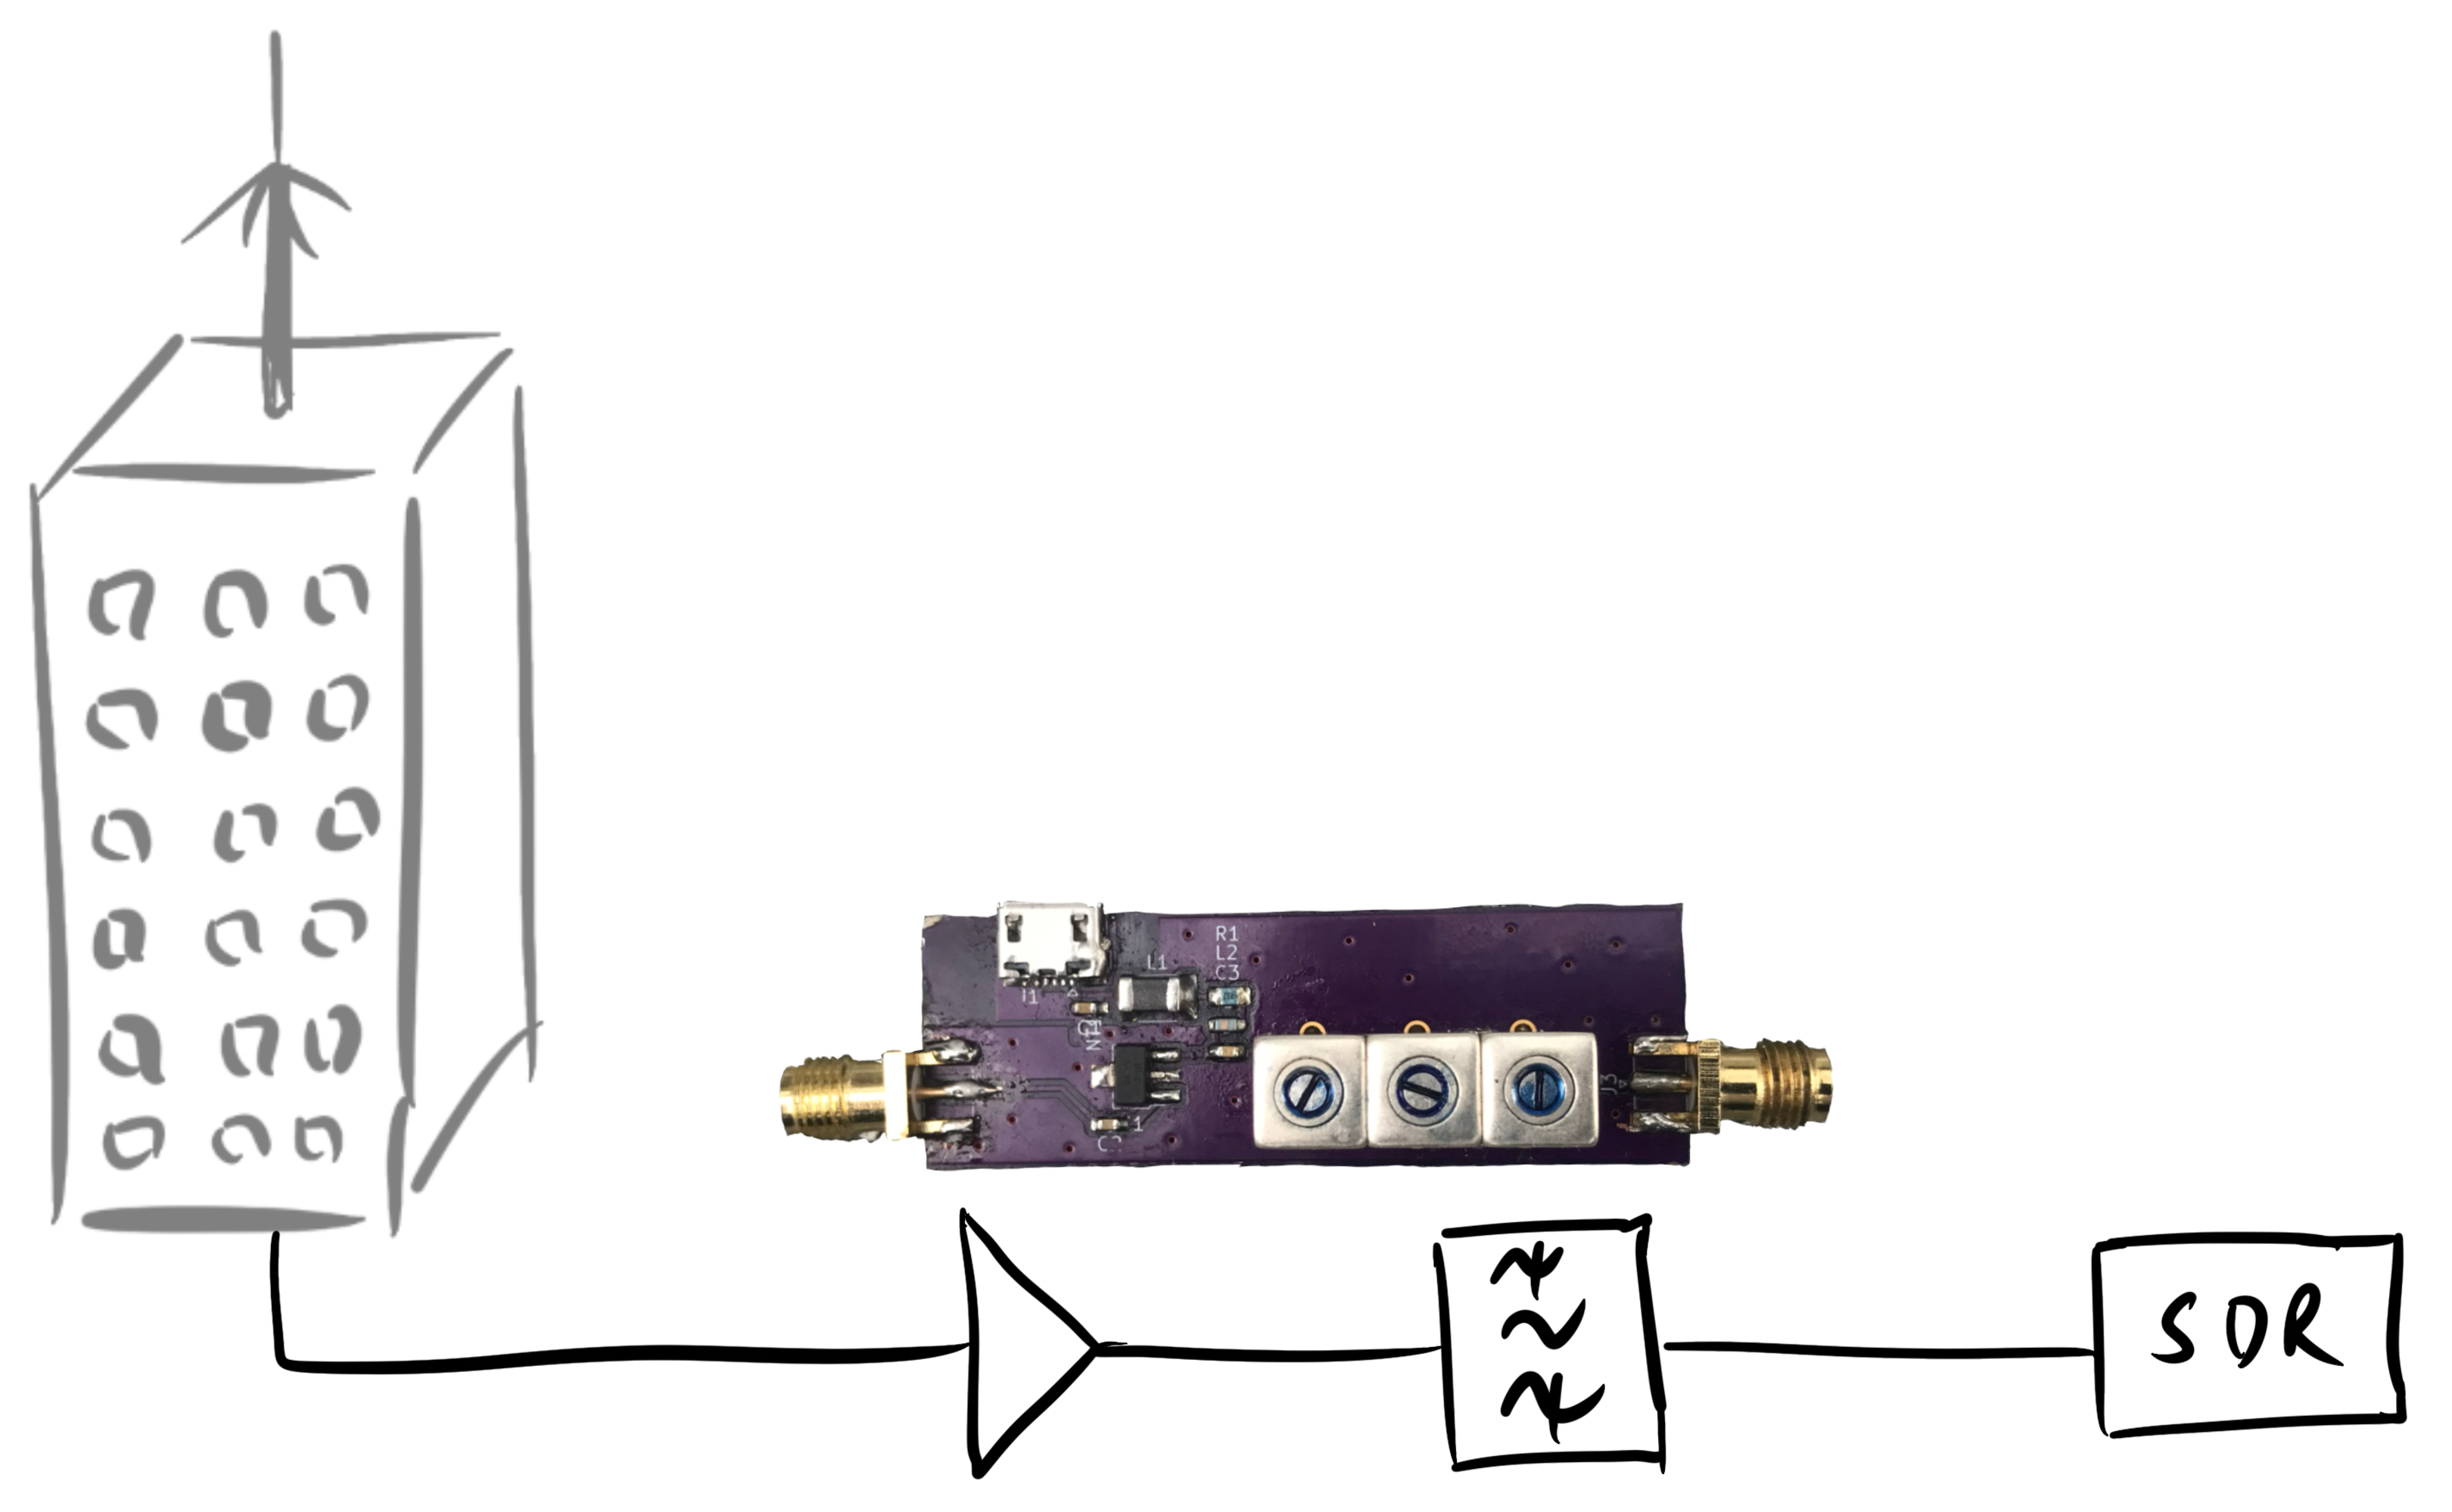
\includegraphics[height=0.65\textheight]{figs/antenna-filter.pdf}
\caption{Schematic overview of the receiver hardware}
\end{figure}
\end{frame}

% =================================================

\begin{frame}
\frametitle{Protocol}
\framesubtitle{VDV 420}
\todo[inline]{This slide is a big todo}
	\begin{itemize}
%		\item which protocol?
%		\item which frequency?
		\item some background on Ampelbeeinflussung and VDV 420 / 426
		\item R09 telegrams of trams and busses standardized in \Colorhref{https://knowhow.vdv.de/documents/420/}{VDV 420}
	\end{itemize}
\end{frame}

% =================================================

\begin{frame}
\frametitle{Protocol}
\framesubtitle{VDV 420 Data}
\begin{itemize}
	\item What data do we receive?
	\begin{itemize}
		\item Tram identification: line number (3 decimal digits), run number (2 decimal digits), destination number (3 digits)
		\item Location: Reporting point (16 bit) which might contain 2 bit registration\_type (Pre-registration, Registraion, De-registration, Doors closed), traffic light id and direction
		\item Other data: Delay ($\pm 7$), train length (until now always zero) etc.
	\end{itemize}
\end{itemize}
\end{frame}

% =================================================

\begin{frame}
\frametitle{Protocol}
\framesubtitle{VDV 420 Data}
\begin{itemize}
	\item Representation of data might be different from the original standard
	\item Dresden: Reporting Point = $((<TRAFFIC\ LIGHT\ ID> *\ 10\ + <DIRECTION>) << 2)\ | <REGISTRATION>$
	\item Tirol: Reporting Point = $((<DIRECTION> *\ 1000\ + <TRAFFIC\ LIGHT\ ID>) << 2)\ | <REGISTRATION>$ \Colorhref{https://www.tirol.gv.at/fileadmin/themen/verkehr/verkehrsplanung/Verkehrsmanagement/Downloads/101022\_PRL\_VLSA-Tirol\_V1.1\_inkl\_Anh01-Anh10.pdf}{}
	%\todo[inline]{represantion of dresden/tirol}
\end{itemize}
\begin{figure}
\centering
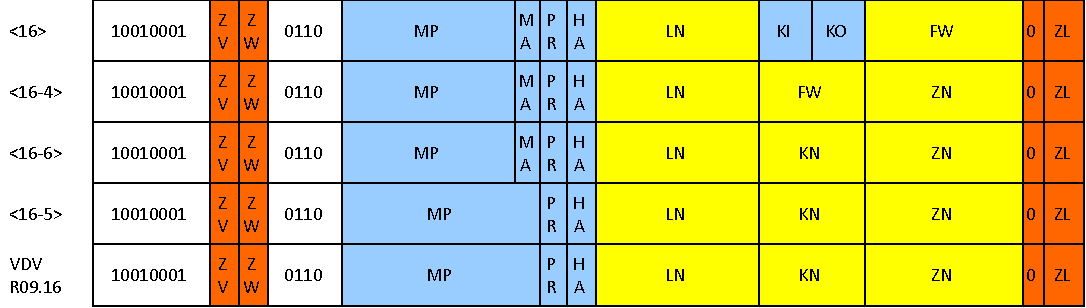
\includegraphics[width=.9\textwidth]{figs/vdv426-r09-variants.pdf}
\caption{\Colorhref{https://knowhow.vdv.de/documents/426/}{VDV 426} specifies different formats for the data fields}
\end{figure}
\end{frame}

% =================================================

\begin{frame}
\frametitle{Protocol}
\framesubtitle{VDV 420 Physical Layer}
\begin{columns}
\column{0.6\linewidth}
\centering
\begin{figure}
\centering
\begin{subfigure}[b]{0.46\textwidth}
	\centering
	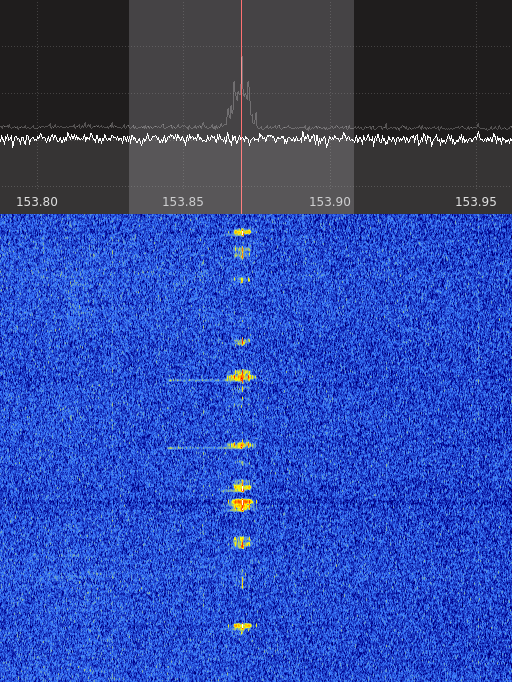
\includegraphics[height=0.65\textheight,width=\textwidth]{figs/spectrum_chemnitz_cropped.png}
\end{subfigure}
\hfill
\begin{subfigure}[b]{0.46\textwidth}
	\centering
	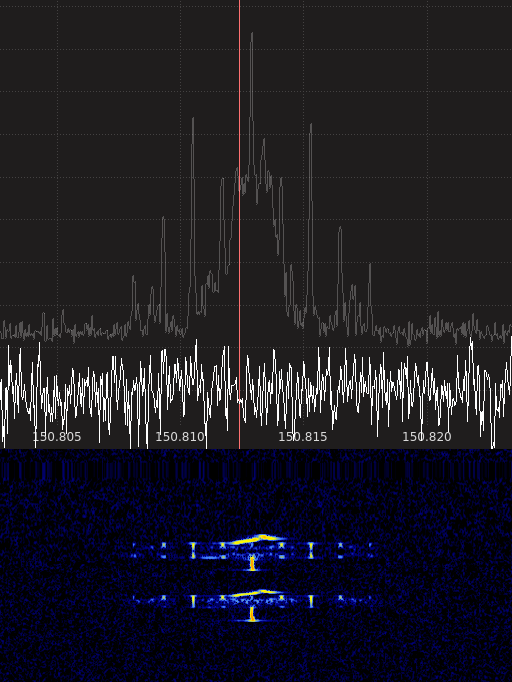
\includegraphics[height=0.65\textheight,width=\textwidth]{figs/spectrum_dresden_cropped.png}
\end{subfigure}
\caption{Screenshots of the bursty transmittion pattern}
\end{figure}
\column{0.4\linewidth}
\begin{itemize}
	\item Bursty transmittion
	\item Minimum Shift Keying with \SI{2400}{Baud}
\end{itemize}
\end{columns}
\end{frame}

% =================================================

\begin{frame}
\frametitle{Protocol}
\framesubtitle{Frequency Identification}
\begin{columns}
\column{.276\linewidth}
\centering
\begin{figure}
	\centering
	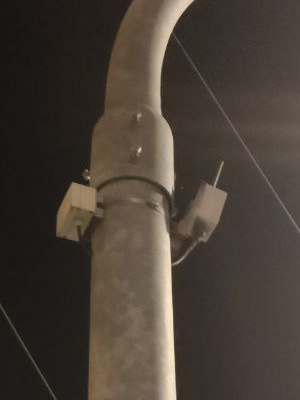
\includegraphics[width=\textwidth]{figs/lsa-antenna.png}
	\caption{Telegram receiver on the right}
\end{figure}
\column{.724\linewidth}
\begin{itemize}
		\item What are the frequency ranges to look for the signal?
		\item Technical documentation of different receivers, i.e. \Colorhref{https://www.piciorgros.com/fileadmin/documents/RBL380.pdf}{RBL-380} or \Colorhref{https://www.img-nordhausen.de/wp-content/uploads/2021/05/DA\_WZLSA\_2-3\_G\_d\_03\_15.pdf}{WZ LSA 2-3/G}, provide these details
		\item Frequency 70cm Band \SI{450}{\MHz} -- \SI{470}{\MHz}		
		\item Frequency 2m Band \SI{146}{\MHz} -- \SI{174}{\MHz}
		\item Frequency 4m Band \SI{68}{\MHz} -- \SI{87.5}{\MHz}
		\item We have a \Colorhref{https://docs.dvb.solutions/chapter\_3\_data\_providers.html}{table of known frequencies}
		\item OSINT: Search for ``R09 frequency <city>''
\end{itemize}
\end{columns}
\end{frame}

% =================================================

\begin{frame}
\frametitle{Protocol}
\framesubtitle{Physical Layer Used in Different Cities}
\begin{figure}
% https://opus4.hbz-nrw.de/opus45-bast/frontdoor/deliver/index/docId/2595/file/V353+BF+Gesamtversion.pdf
% page 25
\begin{columns}
\column{.5\linewidth}
\centering
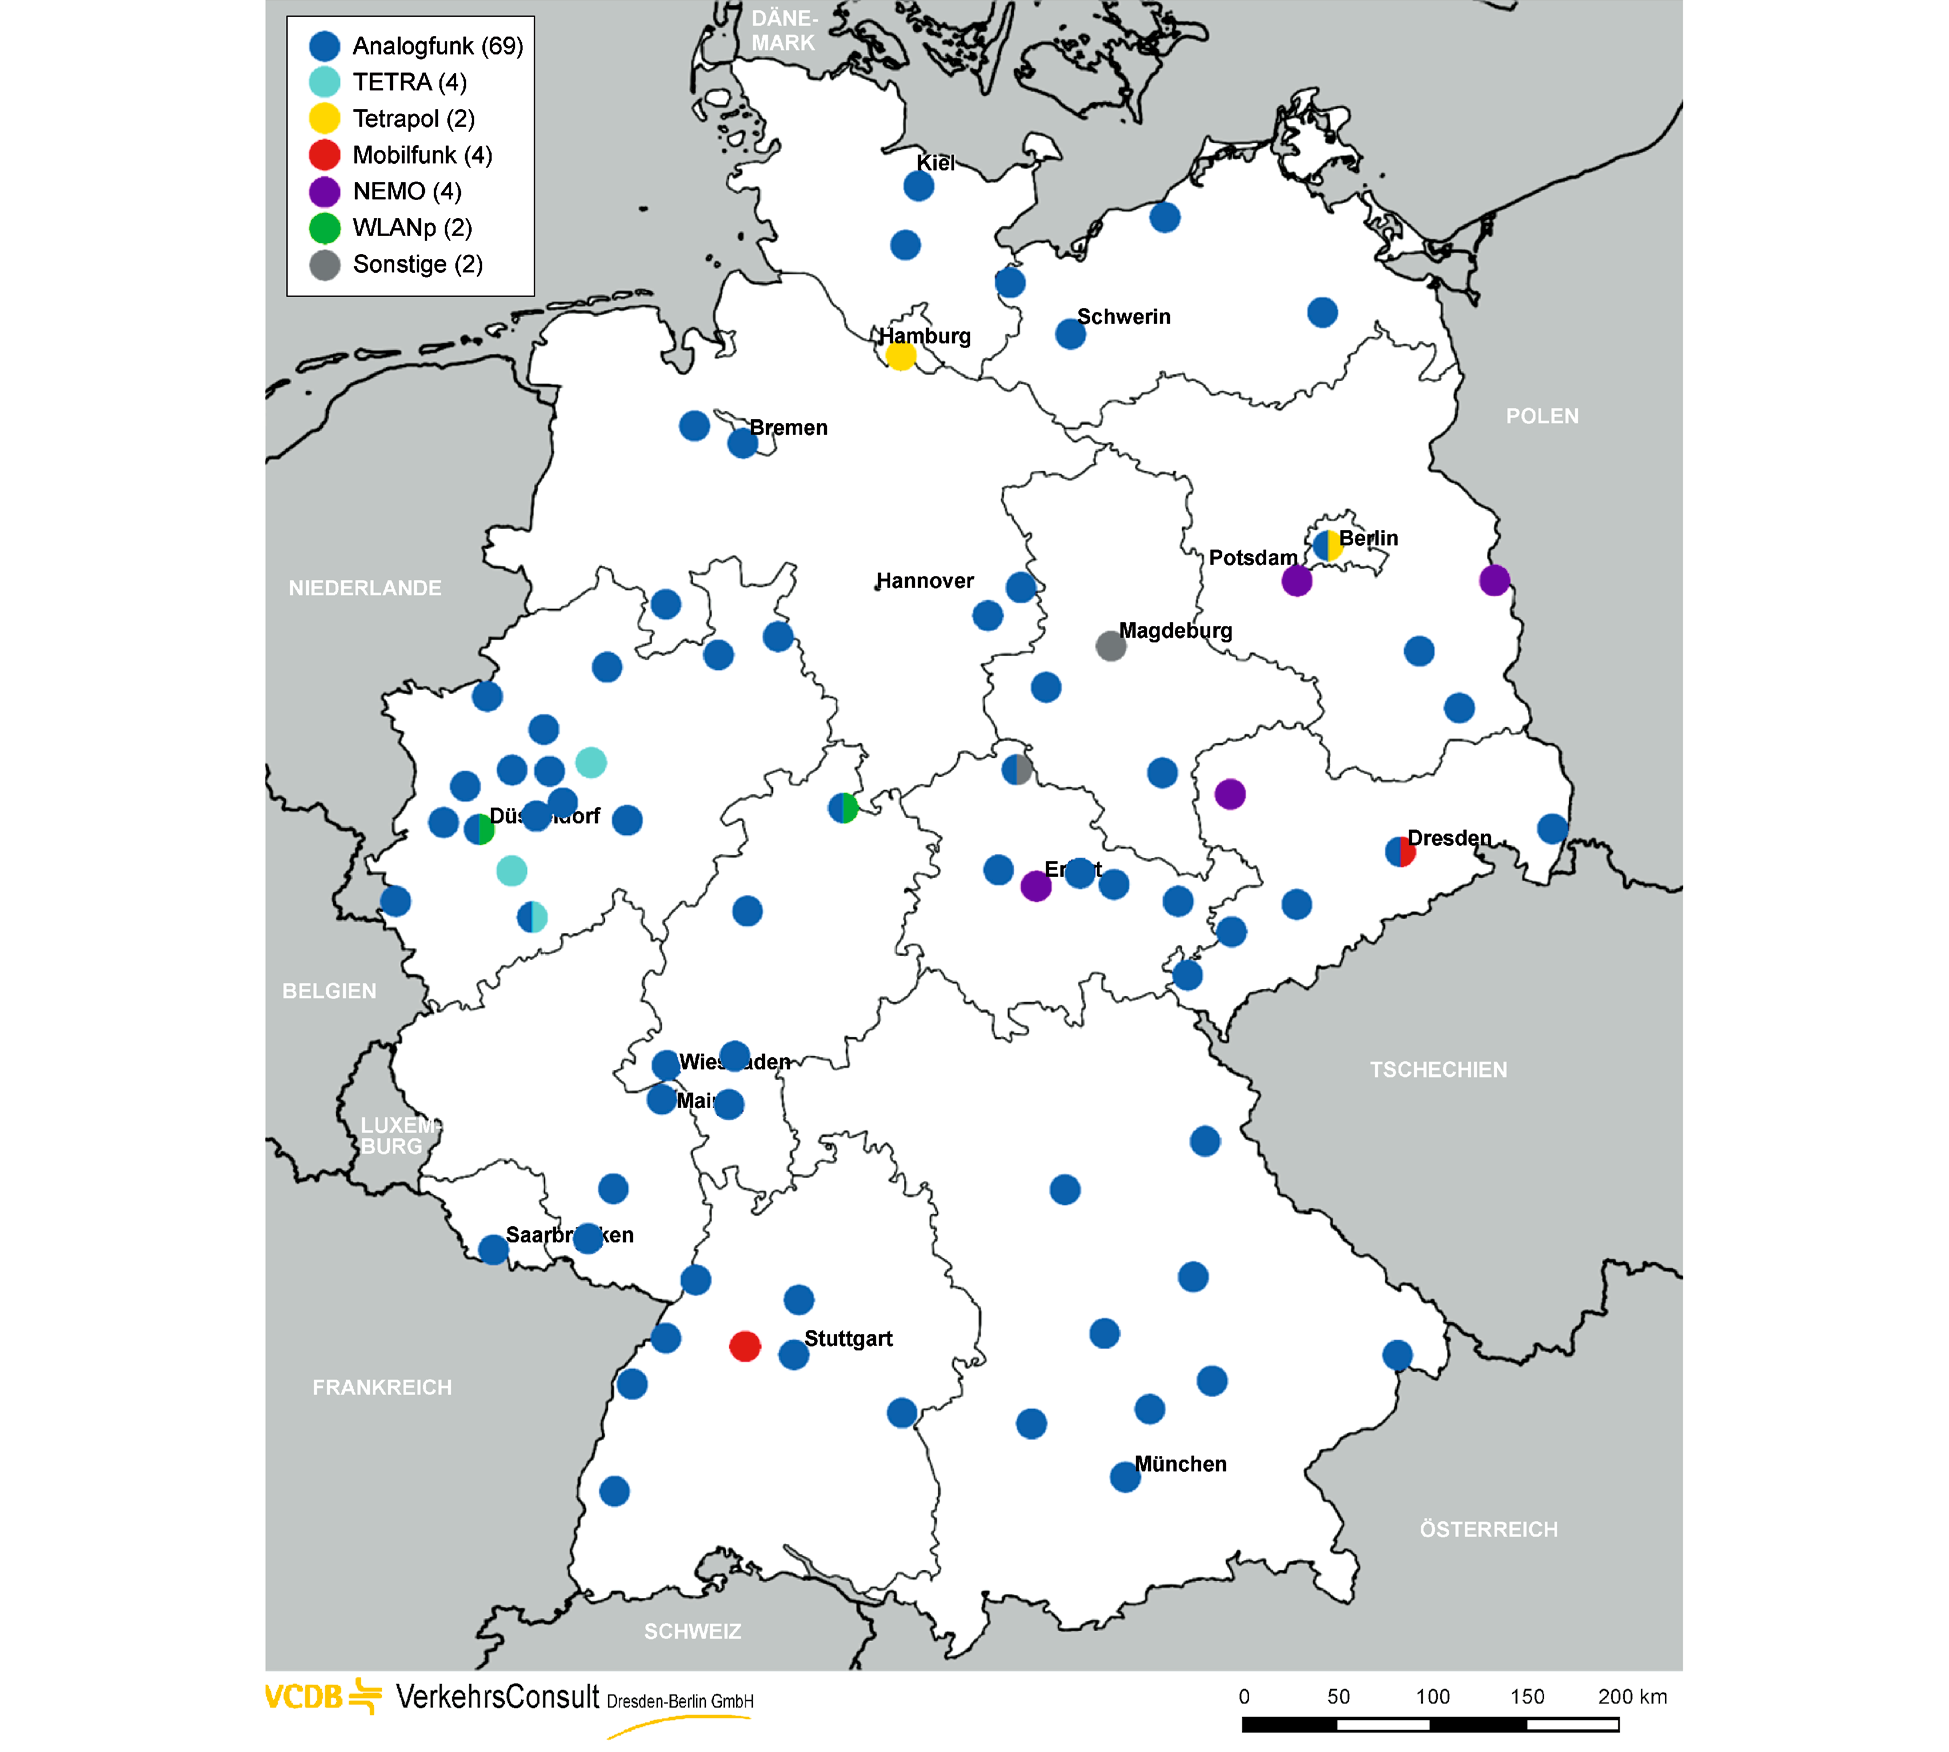
\includegraphics[height=0.8\textheight]{figs/vcdb-map-ampelbeeinflussung.png}
\column{.5\linewidth}
\caption{\Colorhref{https://opus4.hbz-nrw.de/opus45-bast/frontdoor/deliver/index/docId/2595/file/V353+BF+Gesamtversion.pdf}{Map from bast} with selected locations which have traffic lights, controlled by public transport. Blue points use the standard we implemented.}
%\vspace{0.5cm}
\begin{itemize}
	\item Implementations using a different physical layer exsist too, i.e. Berlin with Tetrapol
	\item \Colorhref{https://knowhow.vdv.de/documents/426/}{VDV 426} has more information on this topic
	\item Actual included data doesn't seem to be different
\end{itemize}
\end{columns}
\end{figure}
\end{frame}

% =================================================


% =================================================

\section{Soul Extrating Information \& Mapping }

% =================================================

% For the map we need to know transmission locations.
% No locations in the telegrams, but "reporting points"

% Urbic site leaked quite some junction numbers
% sweatshop => json => first frontend up and running
% By hand doesn't scale, and OSINT is unrelaible source of the info => mapping

% record telegrams and positions => cross reference via time
% nice mobile box, gps tracker everyone has in their pocket nowadays

% run number is important!

% lofi! Several modes of operation.

% Process Now
%Low coverage => box plus phone
% nice stations => just GPS tracks

% Process in da future
% infer run number!
% just a track, with a nice web front

% Far future => infer as much as possible

%%%%%%%%%%%%%%%%%%%%%%%%%%%%%%%%%%%%%%%%%%%%%%%%%%%%%%%%%%%%%%%%%%%
\begin{frame}[fragile]
  \frametitle{the Problem}
  \framesubtitle{Where the Foxtrot Telegram Was Transmitted}

  \begin{columns}
    \column{.6\linewidth}

    \begin{itemize}
      \uncover<1->{\item{R09Telegram doesn't provide map position data}}
      \uncover<1->{\item{location is identified by arbitrary integer reporting\_point}}
      \uncover<2->{\item{To the Google we go!}}
  \end{itemize}

  \column{.4\linewidth}

  \begin{lstlisting}[basicstyle=\scriptsize]
{
  ...
  "reporting_point":8366,
  "junction":209,
  "direction":1,
  "request_status":2,
  ...
}
  \end{lstlisting}

\end{columns}

\end{frame}

%%%%%%%%%%%%%%%%%%%%%%%%%%%%%%%%%%%%%%%%%%%%%%%%%%%%%%%%%%%%%%%%%%%
\begin{frame}
  \frametitle{OSINT Data}
  \framesubtitle{Or Google Your Own LSA ID's}
  \centering
  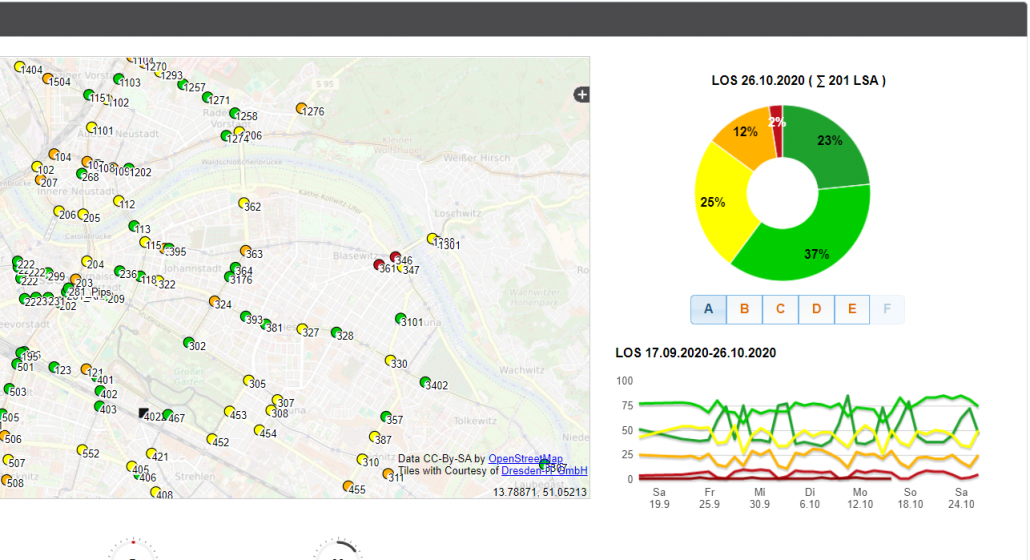
\includegraphics[width=.8\textwidth]{./figs/urbic-osint.png}
\end{frame}

%%%%%%%%%%%%%%%%%%%%%%%%%%%%%%%%%%%%%%%%%%%%%%%%%%%%%%%%%%%%%%%%%%%
\begin{frame}
  \frametitle{Mapping}
  \framesubtitle{JSON Sweatshop, aka Force Your Daughter to Work Day}
  \centering
  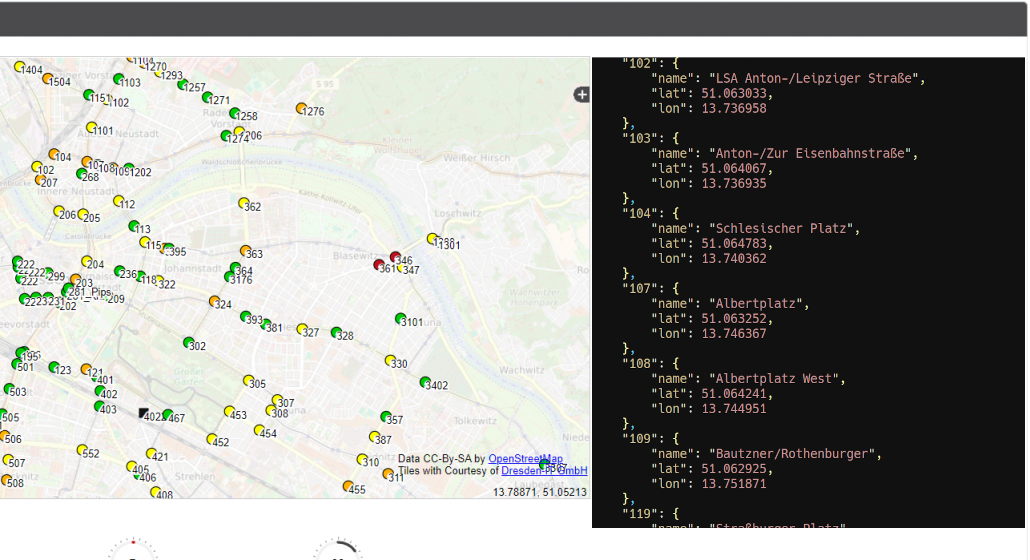
\includegraphics[width=.8\textwidth]{./figs/urbic-osint-json.png}
\end{frame}

%%%%%%%%%%%%%%%%%%%%%%%%%%%%%%%%%%%%%%%%%%%%%%%%%%%%%%%%%%%%%%%%%%%
\begin{frame}
  \frametitle{Mapping}
  \begin{columns}
    \column{.7\linewidth}
    \begin{itemize}
      \item "By Hand" doesn't scale too well
      \item OSINT is unreliable source of information
      \item Junction number corresponds to several reporting points
      \item Need a way to correlate telegrams to map location!
    \end{itemize}
    \column{.3\linewidth}
    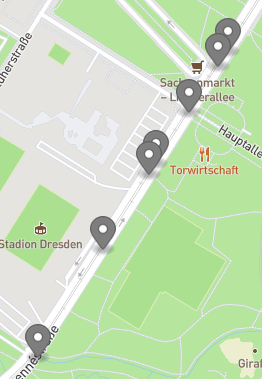
\includegraphics[width=\columnwidth]{./figs/moar_points.png}
  \end{columns}
\end{frame}

%%%%%%%%%%%%%%%%%%%%%%%%%%%%%%%%%%%%%%%%%%%%%%%%%%%%%%%%%%%%%%%%%%%
\begin{frame}
  \frametitle{Dump DVB: Modern WarFerry}
  \framesubtitle{GPS, Puns and Radio}
  \begin{columns}
    \column{.6\linewidth}
      Telegram Recording:
        \begin{itemize}
      \item SDR with a computer in a tupperware
      \item Running off a powerbank
      \item Wartrammer-40k: filters telegrams
    \end{itemize}
      Location Recording: Phone\\
      Correlation: lofi
    \column{.4\linewidth}
    \todo[inline]{nice warferry nudes}
  \end{columns}
\end{frame}

%%%%%%%%%%%%%%%%%%%%%%%%%%%%%%%%%%%%%%%%%%%%%%%%%%%%%%%%%%%%%%%%%%%
\begin{frame}
  \frametitle{Mapping the City}
  \framesubtitle{How it's done now}
  \begin{columns}
    \column{.6\linewidth}
    Bootstraping:
    \begin{itemize}
      \item Go around the city with a warferry
      \item Track your position and line/run number
      \item Correlate the data
    \end{itemize}
    Decent city coverage by radio stations:
    \begin{itemize}
      \item Go around the city
      \item Track your position and line/run number
      \item Correlate the positions to telegrams from the station
    \end{itemize}
    \column{.4\linewidth}
    \todo[inline]{nice warferry picture}
  \end{columns}
\end{frame}

%%%%%%%%%%%%%%%%%%%%%%%%%%%%%%%%%%%%%%%%%%%%%%%%%%%%%%%%%%%%%%%%%%%
\begin{frame}
  \frametitle{Mapping the City, but better}
  \framesubtitle{Stuff that still needs doing}
  \begin{itemize}
    \item In some cities no easy way to get run number => inference from reporting point
    \item "Go around the city" part sucks
    \item Nice gps track submission web thing (together with line number tracking)
  \end{itemize}
\end{frame}


% =================================================

\section{Architecture \& Infra }

% =================================================

% The fucking story

% those people before me thought you the basics about the standard and the protocol and
% how we extract useful information out of the telegrams

% in thematical order
% - what is the current scale of operation
%   - map of stations
%   - plot
%   - with which receivers
% - how do we process data
%   - accurate: radio + telegram decoder
%   - services: just {
%   - lessons learned
% - what do you can get from us
% - what do we achieve examplary calculation
  % - but you can help increase quality as segway into

% =================================================

\usetikzlibrary{calc}
\usetikzlibrary{decorations.pathreplacing,decorations.markings,shapes.geometric}
\tikzset{radiation/.style={{decorate,decoration={expanding waves,angle=90,segment length=4pt}}}}

\lstdefinelanguage{Nix}{
  keywords={true, false},
  keywordstyle=\color{blue}\bfseries,
  ndkeywords={class, export, boolean, throw, implements, import, this},
  ndkeywordstyle=\small \color{darkgray}\bfseries,
  identifierstyle=\scriptsize \color{black},
  sensitive=false,
  comment=[l]{//},
  morecomment=[s]{/*}{*/},
  commentstyle=\color{purple}\ttfamily,
  stringstyle=\color{red}\ttfamily,
  morestring=[b]',
  morestring=[b]",
  basicstyle=\scriptsize,
  %$numbers=left,
  stepnumber=1,
  numbersep=8pt,
  tabsize=4,
  showspaces=false,
  showstringspaces=false
}

\begin{frame}
  \frametitle{Receivers in Operation}

\begin{figure}
\begin{columns}
\column{.5\linewidth}
\centering
  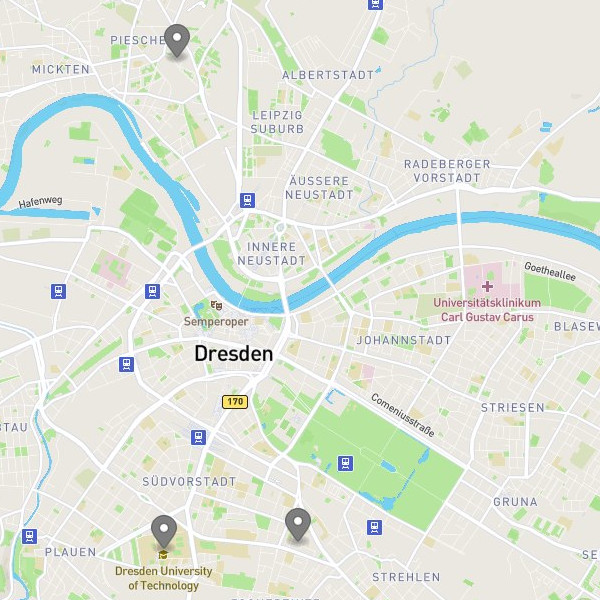
\includegraphics[height=0.65\textheight]{figs/map_dresden.jpg}
  \caption{Receivers in Dresden}
\column{.5\linewidth}
\centering
  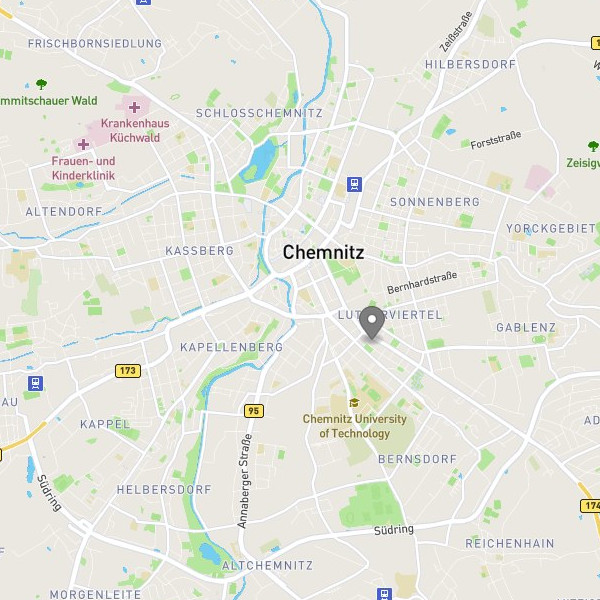
\includegraphics[height=0.65\textheight]{figs/map_chemnitz.jpg}
  \caption{Receivers in Chemnitz}
\end{columns}
\end{figure}

\end{frame}

% =================================================

\begin{frame}
\frametitle{Received Data}

\begin{figure}[h!]
  \begin{center}
    \begin{tikzpicture}[scale=0.6]
      \begin{axis}[
          width=\linewidth,
          grid=major,
          grid style={dashed,gray!30},
          xlabel=Time over 4 days,
          ylabel=Telegrams in 5 minute intervals,
          %x unit=time,
          %y unit=\si{\ampere},
          %legend style={at={(0.5,-0.2)},anchor=north},
          x tick label style={rotate=90,anchor=east},
          xticklabels={,,},
          %xticklabels={day1, day2, day3, day4} TODO: make nice labels
        ]
        \addplot
        table[x=time,y=value,col sep=comma] {figs/rawdata.csv};
      \end{axis}
    \end{tikzpicture}
  \end{center}
\end{figure}


\end{frame}

% =================================================

\begin{frame}
\frametitle{What can we see}

\begin{figure}[h!]
  \begin{center}
    \missingfigure[figwidth=6cm]{Heat Map of Locations}
    \caption{visible reporting points in the city}
  \end{center}
\end{figure}


\end{frame}

% =================================================

\begin{frame}
\frametitle{Converage Estimation}

\begin{figure}
\begin{columns}
\column{.5\linewidth}
\begin{center}
  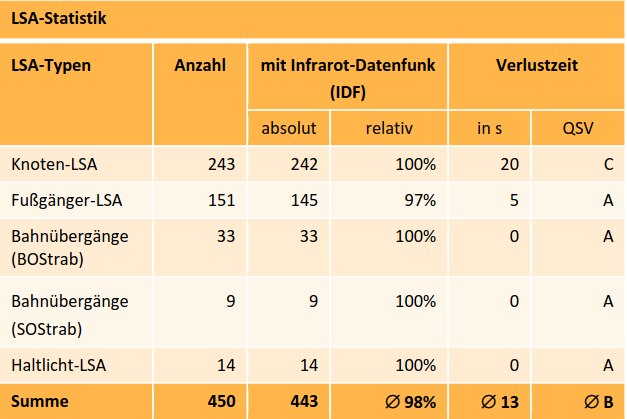
\includegraphics[height=0.6\textheight]{figs/urbic_stops_dresden.jpg}
  \caption{Statistic of traffic lights in dresden from \Colorhref{https://urbic-system.com/wp-content/uploads/2020/10/Qualitaetssicherung-an-Lichtsignalanlagen-aus-Sicht-des-OEPNV-im-urbanen-Umfeld-Kopie.pdf}{urbic 01/2014}}
\end{center}
\column{.5\linewidth}
\raggedright
\vspace{0.5cm}

\begin{itemize}
  \item \todo[inline]{Add query}
  \item See $\approx$ 60\% of the city
\end{itemize}

\end{columns}
\end{figure}

\end{frame}

% =================================================

\begin{frame}
\frametitle{Assembeling a Receiver}

\begin{figure}
\begin{columns}
\column{.5\linewidth}
\begin{center}
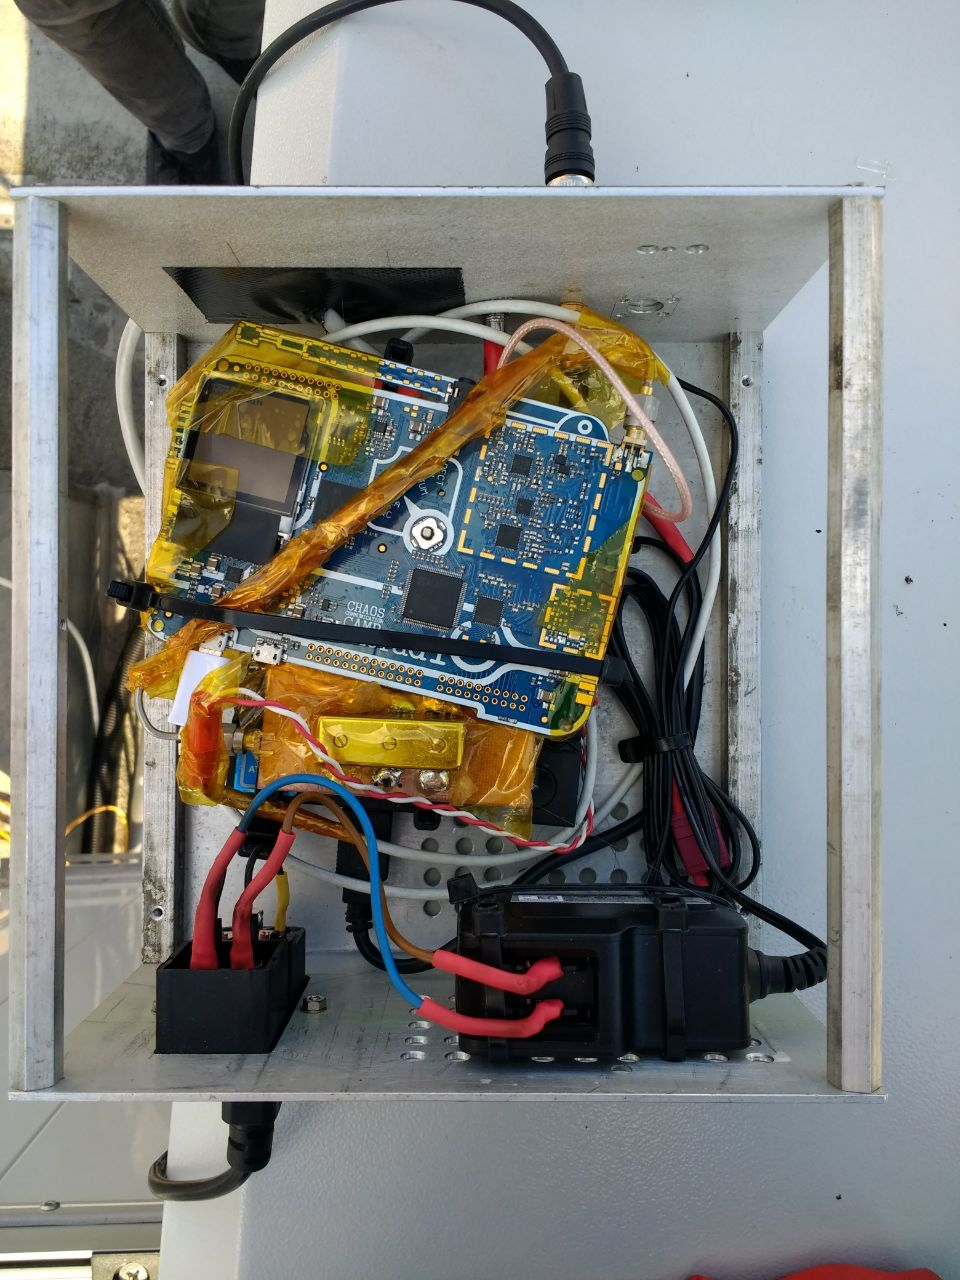
\includegraphics[height=0.7\textheight]{figs/station_barkhausen.jpg}
\end{center}
\column{.5\linewidth}
\raggedright
\caption{\raggedright Station Barkhausenbau}
%\vspace{0.5cm}

\begin{itemize}
	%\item\todo[inline]{make caption allign left}
	%\item\todo[inline]{please provide some details about this station}
  \item GDR powersuply casing (10\euro)
  \item Dell Wyse 3040 (70\euro)
  \item Rad1o Badge (e.g RTL SDR 30\euro)
  \item Hardware Filter (20\euro)
  \item Antenna (15\euro)
  \item Miscellaneous items (15\euro)
  \item Healthy amounts of kapton
\end{itemize}

$\Rightarrow$ ~160\euro \ per Station

\end{columns}
\end{figure}

\end{frame}

% =================================================

\begin{frame}
\frametitle{Receiver}

\begin{figure}
\begin{columns}
\column{.5\linewidth}
\begin{center}
  \begin{tikzpicture}[scale=0.8]
    % Station Box
\filldraw[draw=black,fill=lightgray] (0,3) rectangle (3,-3);

% GNU Radio and Telegram Decoder
\filldraw[draw=black,fill=gray] (0.1,0.8) rectangle (2.9,2.8);
\filldraw[draw=black,fill=gray] (0.1,-0.8) rectangle (2.9,-2.8);

% Data Flow
\draw[->,rounded corners, line width=0.25mm, red] (1.5, 0.8) -- (1.5,-0.8);

% Antenna Drawing
\draw[rounded corners, line width=0.25mm, black] (3, 1.8) -- (4,1.8) -- (4, 4);
\draw[radiation,decoration={angle=45}] (4,4) -- +(180:1);
\draw[radiation,decoration={angle=45}] (4,4) -- +(0:1);

% Labeling
\node[text width=2cm] at (1.5,1.8) {GNU-Radio};
\node[text width=2cm] at (1.5,-1.8) {\centering Telegram Decoder};

\node[text width=0.2cm] at (1.7,0) {\tiny UDP};

    \node[text width=0.2cm] at (3.25,-1.5) {\tiny REST};
    \draw[->,rounded corners, line width=0.25mm, orange] (3, -1.8)  -- (3.5, -1.8);

  \end{tikzpicture}
\end{center}
\column{.5\linewidth}
\raggedright
\vspace{0.5cm}

\begin{itemize}
  \item Region specific encoding depending on special quirks from the city
  \item Currently only parses R09.16 and everything else is recorded as raw-telegram
  \item Authenticates with station UUID and token
\end{itemize}

\end{columns}
\end{figure}

\end{frame}

% =================================================

\begin{frame}
  \frametitle{Server}
  \begin{figure}
    \begin{center}
      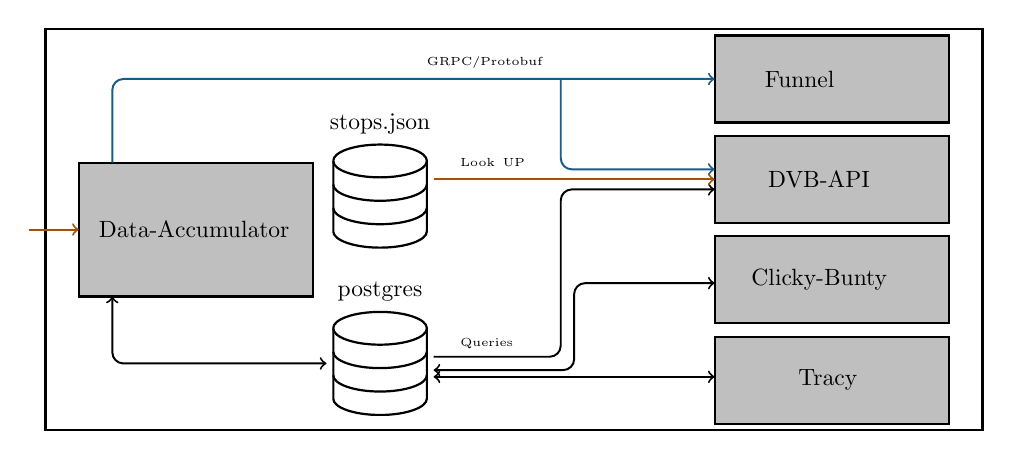
\begin{tikzpicture}[thick,scale=0.85, every node/.style={scale=0.85}]
        \filldraw[draw=black,fill=white] (5,3) rectangle (19,-3);

\filldraw[draw=black,fill=lightgray] (5.5,1) rectangle (9,-1);
\node[database,label=above:postgres,database radius=0.7cm,database segment height=0.35cm] at (10,-2) {};
\node[database,label=above:stops.json,database radius=0.7cm,database segment height=0.35cm] at (10,0.5) {};

% DataAccm <-> Postgres
\draw[<->,rounded corners, line width=0.25mm] (6, -1)  -- (6,-2) -- (9.2,-2);
%\draw[->,rounded corners, line width=0.25mm] (9.2, -1.9)  -- (6.1,-1.9) -- (6.1,-1);

% User Facing Services
\filldraw[draw=black,fill=lightgray] (15,2.9) rectangle (18.5,1.6);
\filldraw[draw=black,fill=lightgray] (15,1.4) rectangle (18.5,0.1);
\filldraw[draw=black,fill=lightgray] (15,-0.1) rectangle (18.5,-1.4);
\filldraw[draw=black,fill=lightgray] (15,-1.6) rectangle (18.5,-2.9);

% GRPC Arrows
% 1f77b4 31 119 180
\draw[->,rounded corners, draw={rgb:red,31;green,119;blue,180}, line width=0.25mm] (6, 1)  -- (6,2.25) -- (15,2.25);
\draw[->,rounded corners, draw={rgb:red,31;green,119;blue,180}, line width=0.25mm] (12.7, 2.25)  -- (12.7,0.9) -- (15,0.9);

% Postgres Arrows
% Tracy
\draw[<->,rounded corners, line width=0.25mm] (10.8, -2.2)  -- (15,-2.2);
%\draw[->,rounded corners, line width=0.25mm] (15, -2.3)  -- (10.8,-2.3);
% Clicky-Bunty-Server
\draw[<->,rounded corners, line width=0.25mm] (15, -0.8)  -- (12.9, -0.8) -- (12.9, -2.1) -- (10.8,-2.1);
%\draw[->,rounded corners, line width=0.25mm] (10.8, -2)  -- (12.8, -2) -- (12.8, -0.7) -- (15,-0.7);
% DVB-API
\draw[->,rounded corners, line width=0.25mm] (10.8, -1.9)  -- (12.7, -1.9) -- (12.7, 0.6) -- (15, 0.6);

% Labeling
\node[text width=3cm] at (7.3,0) {Data-Accumulator};
\node[text width=2cm] at (16.75,2.25) {Funnel};
\node[text width=2cm] at (16.8,0.75) {DVB-API};
\node[text width=2.5cm] at (16.8,-0.75) {Clicky-Bunty};
\node[text width=1cm] at (16.75,-2.25) {Tracy};

% Look Ups
\draw[->,rounded corners, draw={rgb:red,255;green,127;blue,14}, line width=0.25mm] (10.8, 0.75)  -- (15, 0.75);

% Labeling Arrows
\node[text width=2cm] at (11.7,2.5) {\tiny GRPC/Protobuf};
\node[text width=1cm] at (11.7,1) {\tiny Look UP};
\node[text width=1cm] at (11.7, -1.7) {\tiny Queries};

% ff7f0e 255 127 14
\draw[->,rounded corners, draw={rgb:red,255;green,127;blue,14}, line width=0.25mm] (4.75, 0)  -- (5.5, 0);

      \end{tikzpicture}
    \end{center}
  \end{figure}
\end{frame}

% =================================================

\begin{frame}
\frametitle{Architecture}

% Funnel
% DVB-API
% Clicky-Bunty
% Tracy
\begin{tikzpicture}[thick,scale=0.55, every node/.style={scale=0.65}]

% Station Box
\filldraw[draw=black,fill=lightgray] (0,3) rectangle (3,-3);

% GNU Radio and Telegram Decoder
\filldraw[draw=black,fill=gray] (0.1,0.8) rectangle (2.9,2.8);
\filldraw[draw=black,fill=gray] (0.1,-0.8) rectangle (2.9,-2.8);

% Data Flow
\draw[->,rounded corners, line width=0.25mm, red] (1.5, 0.8) -- (1.5,-0.8);

% Antenna Drawing
\draw[rounded corners, line width=0.25mm, black] (3, 1.8) -- (4,1.8) -- (4, 4);
\draw[radiation,decoration={angle=45}] (4,4) -- +(180:1);
\draw[radiation,decoration={angle=45}] (4,4) -- +(0:1);

% Labeling
\node[text width=2cm] at (1.5,1.8) {GNU-Radio};
\node[text width=2cm] at (1.5,-1.8) {\centering Telegram Decoder};

\node[text width=0.2cm] at (1.7,0) {\tiny UDP};

\filldraw[draw=black,fill=white] (5,3) rectangle (19,-3);

\filldraw[draw=black,fill=lightgray] (5.5,1) rectangle (9,-1);
\node[database,label=above:postgres,database radius=0.7cm,database segment height=0.35cm] at (10,-2) {};
\node[database,label=above:stops.json,database radius=0.7cm,database segment height=0.35cm] at (10,0.5) {};

% DataAccm <-> Postgres
\draw[<->,rounded corners, line width=0.25mm] (6, -1)  -- (6,-2) -- (9.2,-2);
%\draw[->,rounded corners, line width=0.25mm] (9.2, -1.9)  -- (6.1,-1.9) -- (6.1,-1);

% User Facing Services
\filldraw[draw=black,fill=lightgray] (15,2.9) rectangle (18.5,1.6);
\filldraw[draw=black,fill=lightgray] (15,1.4) rectangle (18.5,0.1);
\filldraw[draw=black,fill=lightgray] (15,-0.1) rectangle (18.5,-1.4);
\filldraw[draw=black,fill=lightgray] (15,-1.6) rectangle (18.5,-2.9);

% GRPC Arrows
% 1f77b4 31 119 180
\draw[->,rounded corners, draw={rgb:red,31;green,119;blue,180}, line width=0.25mm] (6, 1)  -- (6,2.25) -- (15,2.25);
\draw[->,rounded corners, draw={rgb:red,31;green,119;blue,180}, line width=0.25mm] (12.7, 2.25)  -- (12.7,0.9) -- (15,0.9);

% Postgres Arrows
% Tracy
\draw[<->,rounded corners, line width=0.25mm] (10.8, -2.2)  -- (15,-2.2);
%\draw[->,rounded corners, line width=0.25mm] (15, -2.3)  -- (10.8,-2.3);
% Clicky-Bunty-Server
\draw[<->,rounded corners, line width=0.25mm] (15, -0.8)  -- (12.9, -0.8) -- (12.9, -2.1) -- (10.8,-2.1);
%\draw[->,rounded corners, line width=0.25mm] (10.8, -2)  -- (12.8, -2) -- (12.8, -0.7) -- (15,-0.7);
% DVB-API
\draw[->,rounded corners, line width=0.25mm] (10.8, -1.9)  -- (12.7, -1.9) -- (12.7, 0.6) -- (15, 0.6);

% Labeling
\node[text width=3cm] at (7.3,0) {Data-Accumulator};
\node[text width=2cm] at (16.75,2.25) {Funnel};
\node[text width=2cm] at (16.8,0.75) {DVB-API};
\node[text width=2.5cm] at (16.8,-0.75) {Clicky-Bunty};
\node[text width=1cm] at (16.75,-2.25) {Tracy};

% Look Ups
\draw[->,rounded corners, draw={rgb:red,255;green,127;blue,14}, line width=0.25mm] (10.8, 0.75)  -- (15, 0.75);

% Labeling Arrows
\node[text width=2cm] at (11.7,2.5) {\tiny GRPC/Protobuf};
\node[text width=1cm] at (11.7,1) {\tiny Look UP};
\node[text width=1cm] at (11.7, -1.7) {\tiny Queries};

% ff7f0e 255 127 14
\draw[->,rounded corners, draw={rgb:red,255;green,127;blue,14}, line width=0.25mm] (4.75, 0)  -- (5.5, 0);


% Station Box
\filldraw[draw=black,fill=white] (21,3) rectangle (24,-3);

% GNU Radio and Telegram Decoder
\filldraw[draw=black,fill=lightgray] (21.1,0.1) rectangle (23.9,2.9);
\filldraw[draw=black,fill=lightgray] (21.1,-0.1) rectangle (23.9,-1.4);
\filldraw[draw=black,fill=lightgray] (21.1,-1.6) rectangle (23.9,-2.9);

% Labeling
\node[text width=2cm] at (23,1.5) {Map};
\node[text width=2cm] at (23,-0.75) {Click};
\node[text width=2cm] at (23,-2.25) {Tracy};

\draw[->,rounded corners, draw={rgb:red,255;green,127;blue,14}, line width=0.25mm] (18.5, 2.25)  -- (21, 2.25);

\draw[->,rounded corners, draw={rgb:red,255;green,127;blue,14}, line width=0.25mm] (18.5, 0.75)  -- (21, 0.75);

\draw[<->,rounded corners, draw={rgb:red,255;green,127;blue,14}, line width=0.25mm] (21, -0.7)  -- (18.5, -0.7);
%\draw[->,rounded corners, draw={rgb:red,255;green,127;blue,14}, line width=0.25mm] (18.5, -0.8)  -- (21, -0.8);

\draw[<->,rounded corners, draw={rgb:red,255;green,127;blue,14}, line width=0.25mm] (21, -2.2)  -- (18.5, -2.2);
%\draw[->,rounded corners, draw={rgb:red,255;green,127;blue,14}, line width=0.25mm] (18.5, -2.3)  -- (21, -2.3);


\node[text width=0.1cm] at (19.5,1) {\tiny REST};
\node[text width=0.1cm] at (19.5,-2) {\tiny REST};
\node[text width=0.1cm] at (19.5,2.5) {\tiny SOCKET};
\node[text width=0.1cm] at (19.5,-0.5) {\tiny SOCKET};


\node[text width=0.2cm] at (4,0.2) {\tiny REST};
\draw[->,rounded corners, line width=0.25mm, orange] (3, -1.8)  -- (4,-1.8) -- (4,0) -- (5, 0);

\end{tikzpicture}

\end{frame}

%TODO: Friendship Ended with Influx

% =================================================

\begin{frame}
\frametitle{Throughput}

\begin{figure}[h!]
  \begin{center}
    \begin{tikzpicture}[scale=0.6]
      \begin{axis}[
          width=\linewidth,
          grid=major,
          grid style={dashed,gray!30},
          xlabel=Benchmark over 5 mins,
          ylabel=Telegrams per Second,
          %x unit=time,
          %y unit=\si{\ampere},
          %legend style={at={(0.5,-0.2)},anchor=north},
          x tick label style={rotate=90,anchor=east},
          xticklabels={,,},
          %xticklabels={day1, day2, day3, day4} TODO: make nice labels
        ]
        \addplot
        table[x=time,y=send,col sep=comma] {figs/benchmark.csv};
        \addplot
        table[x=time,y=receive,col sep=comma,color=red] {figs/benchmark.csv};
      \end{axis}
    \end{tikzpicture}
  \end{center}
\end{figure}


\end{frame}

% =================================================

\begin{frame}
  \frametitle{Technical Loans}
  \framesubtitle{Lessons Learned}

\begin{figure}
\begin{columns}
\column{.5\linewidth}
\begin{center}

\includegraphics[height=0.65\textheight]{figs/meme_postgres_influx.png}
\end{center}
\column{.5\linewidth}
\raggedright
\vspace{0.5cm}

\begin{itemize}
  \item Influx
        \begin{itemize}
          \item Database dumps costs 14GB of RAM
          \item Server died hourly
        \end{itemize}
    \item Single point of truth
    \begin{itemize}
        \item Implement Protocols in Libraries which is then used by both parties.
    \end{itemize}
    \item Hardware homogenity
\end{itemize}
\end{columns}
\end{figure}

\end{frame}

% =================================================

\begin{frame}[fragile]
\frametitle{Data We Currently Provide}
\framesubtitle{Funnel: Websocket}
\begin{figure}
\begin{columns}
  \column{.5\linewidth}
  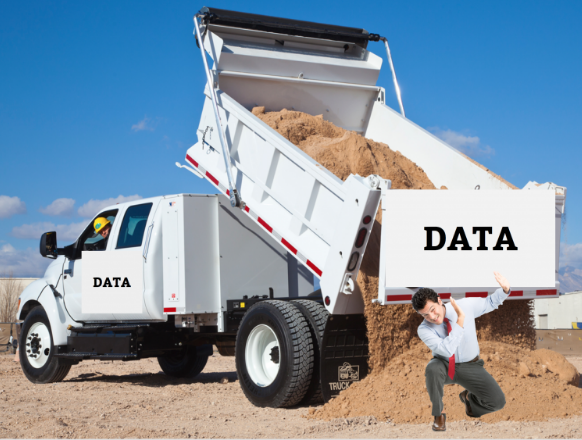
\includegraphics[height=0.65\textheight]{figs/data_dump.png}
\column{.5\linewidth}
\raggedright
\vspace{0.5cm}

\begin{itemize}
  \item 7.7 million telegrams are already recorded
  \item hourly and daily dumps can be fetched from \url{https://files.dvb.solutions}
\end{itemize}
\end{columns}
\end{figure}
\end{frame}
% =================================================

\begin{frame}[fragile]
\frametitle{Data we Currently Provide}
\framesubtitle{Funnel: Websocket}
\begin{figure}
\begin{columns}
  \column{.5\linewidth}
\begin{lstlisting}[basicstyle=\scriptsize]
{
  "time":1662932144,
  "station":"97d028ec-43e2-4473-...",
  "region":0,
  "telegram_type":16,
  "reporting_point":8366,
  "junction":209,
  "direction":1,
  "request_status":2,
  "delay":0,
  "priority":0,
  "direction_request":0,
  "line":4,
  "run_number":9,
  "destination_number":31,
  "train_length":0
}
\end{lstlisting}
\column{.5\linewidth}
\raggedright
\vspace{0.5cm}

\begin{itemize}
  \item \url{https://socket.dvb.solutions}
  \item Configurable Filters (region, line, junction)
  \item Deduplicated
  \item Very raw
\end{itemize}
\end{columns}
\end{figure}
\end{frame}

% =================================================

\begin{frame}[fragile]
\frametitle{Data We Currently Provide}
\framesubtitle{stop.json \& graph.json}

  \begin{itemize}
    \item \url{https://map.dvb.solutions/stop/<region id>.json}
    \item \url{https://map.dvb.solutions/stop/all.json}
    \item \url{https://map.dvb.solutions/graph/<region id>.json}
    \item \url{https://map.dvb.solutions/graph/all.json}
  \end{itemize}
\end{frame}
% =================================================

\begin{frame}[fragile]
\frametitle{Data We Currently Provide}
\framesubtitle{REST DVB-API}

\begin{itemize}
     \item \url{https://api.dvb.solutions}
     \item \textbf{GET  /vehicles/0/all}
     \item \textbf{POST /vehicles/0/query}
     \item \textbf{POST /network/0/estimated\_travel\_time}
     \item \textbf{POST /static/0/coordinates}
  \end{itemize}
\end{frame}

% =================================================


% =================================================

\section{Call for Action}

% =================================================

\begin{frame}
\frametitle{The Project is Huge you can Help !}


\begin{figure}
\begin{columns}
\column{.5\linewidth}
\centering
  
\includegraphics[height=0.8\textheight]{figs/bob_ross_wants_you.jpg}
\column{.5\linewidth}
\centering
\begin{itemize}
  \item Frontend
        \begin{itemize}
          \item \textbf{Tofu}: landing page (TECHNOLOGY OPEN)
          \item \textbf{Tracy}: Mapping Assitent (TECHNOLOGY OPEN)
          \item \textbf{Click}: User + Station Managment (elm-lang)
          \item \textbf{Windshield} Live Map
        \end{itemize}
  \item Setup Stations
  \item Map your City
  \item Find Frequencies
  \item Test Images on new Hardware
  \item Give us Roof Access
\end{itemize}
\end{columns}
\end{figure}


\end{frame}

% =================================================

\section{Questions}

\end{document}
